\cotefile{142}
\scanpage{52}
\mspage{\unsure{6}}
Je vais introduire, dans la sphère $\widetilde\Sigma$ dont le degré de connexion est 0, cinq ouverts, pris aussi grands que possible, qui soient simplement connexes -- obtenus en pratiquant des ``coupures'' qui relient entre eux les \deleted{trois} bords $U_i$ des trois ``trous'' \deleted{$\unsure{\Sigma}$}. On pose
\figure{
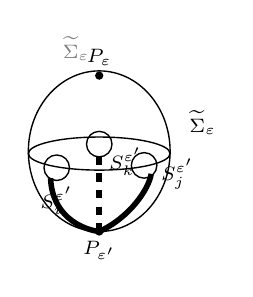
\begin{tikzpicture}[x=.6cm,y=.6cm,every node/.style={font=\scriptsize},line width=.5pt]
\draw (0,0) ellipse (1.5 and 1.7);
\draw (0,-.05) ellipse (1.5 and .35);
\draw (-.9,-.35) circle (.27); \draw (0,.15) circle (.27); \draw (.95,-.3) circle (.27);
\draw[line width=2pt] (-1.03,-.57) .. controls (-1,-1.35) and (-.4,-1.65) .. (0,-1.7) .. controls (.65,-1.4) and (1.05,-.8) .. (1.1,-.48);
\draw[line width=2pt,dashed] (0,-.12)--(0,-1.7);
\fill (0,1.6) circle (1.5pt); \fill (0,-1.7) circle (1.5pt);
\node[above] at (0,1.6) {$P_\varepsilon$}; \node[above left,gray] at (0,1.7) {$\widetilde\Sigma_\varepsilon$};
\node[below] at (0,-1.7) {$P_{\varepsilon'}$};
\node[right] at (0,-.22) {$S_k^{\varepsilon'}$}; \node[below] at (-.9,-.55) {$S_i^{\varepsilon'}$}; \node[right] at (1.1,-.48) {$S_j^{\varepsilon'}$};
\node[right] at (1.7,.6) {$\widetilde\Sigma_\varepsilon$};
\end{tikzpicture}
}
\[
(27)\quad\left\{\begin{aligned}
\widetilde\Sigma_\varepsilon&=\widetilde\Sigma\setminus\bigcup_{i\in J}\operatorname{supp}d_i^\varepsilon \qquad\varepsilon\in\uline{\varepsilon}\\
\widetilde\Sigma_i&=\widetilde\Sigma\setminus\bigcup_{\substack{j\in J\setminus\{i\}\\\deleted{\omega\in\uline{\omega}}}}\deleted{\operatorname{supp}}b_i^{\deleted{\unsure{\omega}}}
\end{aligned}\right.
\]
\margin{(où $b_i=\operatorname{supp}\widetilde b_i^\omega$\newline
\deleted{$=\operatorname{supp}c_i^\omega\cup\operatorname{supp}c_i^{\omega'}$}\newline
$=\operatorname{supp}c_i^\omega\cup\operatorname{supp}c_i^{\omega'}$)}
\figure{
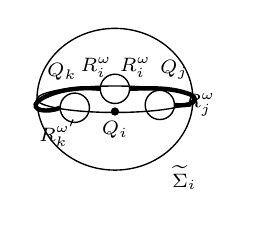
\begin{tikzpicture}[x=.6cm,y=.6cm,every node/.style={font=\scriptsize},line width=.5pt]
\draw (0,0) ellipse (1.65 and 1.5);
\draw (0,0) ellipse (1.65 and .28);
\draw (-.85,-.18) circle (.31); \draw (0,.22) circle (.31); \draw (.95,-.12) circle (.31);
\draw[line width=1.6pt] (-.31,.22) .. controls (-.8,.27) and (-1.35,.18) .. (-1.64,-.05) .. controls (-1.8,-.23) and (-1.45,-.3) .. (-1.16,-.18);
\draw[line width=1.6pt] (.31,.22) .. controls (.8,.24) and (1.2,.25) .. (1.6,.1) .. controls (1.85,-.03) and (1.55,-.17) .. (1.26,-.12);
\fill (0,-.26) circle (1.5pt); \node[below] at (0,-.26) {$Q_i$};
\node[above] at (-1.12,.2) {$Q_k$}; \node[above] at (1.25,.22) {$Q_j$};
\node[above] at (-.4,.25) {$R_i^{\omega}$}; \node[above] at (.43,.25) {$R_i^\omega$};
\node[below] at (-1.2,-.22) {$R_k^{\omega'}$}; \node[right] at (1.26,-.12) {$R_j^\omega$};
\node[below right] at (1,-1.2) {$\widetilde\Sigma_i$};
\end{tikzpicture}
}
Ce sont bien des ouverts \deleted{de $\Sigma$} \inserted{connexes et} simplement connexes de la sphère à trous $\widetilde\Sigma$ (car le complémentaire est connexe. On dit que $P_\omega$ est le \uline{centre} de $\widetilde\Sigma_\omega$, $Q_i$ le \uline{centre} de $\widetilde\Sigma_i$.
\margin{ce sont des ouverts denses, et pour cette raison connexes...}
On pose
\[
(28)\quad\left\{\begin{aligned}
\Pi_\varepsilon&=\Pi_1(\widetilde\Sigma,\widetilde\Sigma_\varepsilon)\simeq\Pi_1(\Sigma^*,\Sigma_\varepsilon^*)\simeq\Pi_1(\Sigma^*,P_\varepsilon)\\
\Pi_i&=\Pi_1(\widetilde\Sigma,\widetilde\Sigma_i)=\Pi_1(\Sigma^*,\Sigma_i^*)\simeq\Pi_1(\Sigma^*,Q_i)
\end{aligned}\right.
\]
en faisant les identifications impliquées par ces formules. \deleted{\unsure{De}} Pour tt $x\in\widetilde\Sigma_\omega$ resp. $x\in\widetilde\Sigma_i$, on pose
\[
(29)\quad\left\{\begin{aligned}
\varphi_{\varepsilon,x}\text{ ou }\varphi_\omega&:\Pi_\varepsilon\xrightarrow{\sim}\Pi_1(\widetilde\Sigma,x)\quad(\simeq\Pi_1(\Sigma^*,x)\text{ si }x\in\Sigma^*)\\
\text{resp.}\ \varphi_{i,x}\text{ ou }\varphi_i&:\Pi_i\xrightarrow{\sim}\Pi_1(\widetilde\Sigma,x)\qquad\text{--}
\end{aligned}\right.
\]
\margin{Les $\varphi$ sont appelés \uline{isom} \uline{de} \uuline{transition}.}
\margin{51}

\scanpage{53}
\mspage{6}
L'isom. canonique déduit de l'inclusion.

On a de plus des isomorphismes canoniques
\[
(30)\quad\left\{\begin{aligned}
\varphi_{i\varepsilon}&:\Pi_\omega\longrightarrow\Pi_i\qquad\text{défini par }c_i^\varepsilon:P_\varepsilon\longrightarrow Q_i\\
\varphi_{\varepsilon i}&:\Pi_i\longrightarrow\Pi_\omega\qquad\text{---}\qquad(c_i^\varepsilon)^{-1}:Q_i\longrightarrow P_\varepsilon
\end{aligned}\right.
\]
\margin{\uline{NB} on a $\varphi_{i\varepsilon}=\varphi_{Q_i,\varepsilon}$, $\varphi_{\varepsilon i}=\varphi_{P_\varepsilon,i}$.}
Par ces isom., les $\Pi_\varepsilon,\Pi_i$ sont reliés de façon transitive, mais bien entendu pas par un syst. transitif d'isomorphismes -- au contraire, les autom. d'un des groupes $\Pi_\varepsilon,\Pi_i$ obtenus en composant des isoms (30) suivant des chemins fermés sur le graphe
\figure{
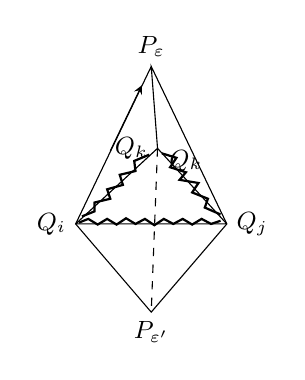
\begin{tikzpicture}[x=.8cm,y=.8cm,>=stealth,every node/.style={font=\small}]
\coordinate (P) at (0,2.5);\coordinate (M) at (0,-1.4);\coordinate (I) at (-1.2,0);\coordinate (J) at (1.2,0);\coordinate (K) at (.1,1.2);
\draw (P)--(I)--(M)--(J)--(P)--(K);
\draw[dashed] (K)--(M);
\draw[->] (-.65,1.16)--(-.15,2.2);
\draw (I)--(J) (I)--(K)--(J);
\draw[thick] (-1.15,.02)--(-1,.08)--(-.85,-.01)--(-.7,.08)--(-.55,-.01)--(-.4,.09)--(-.25,0)--(-.1,.08)--(.05,-.02)--(.2,.08)--(.35,0)--(.5,.08)--(.65,-.01)--(.8,.08)--(.95,0)--(1.1,.05);
\draw[thick] (-1.1,.12)--(-.9,.2)--(-.9,.34)--(-.65,.4)--(-.7,.55)--(-.45,.62)--(-.5,.78)--(-.25,.84)--(-.27,1)--(-.03,1.1);
\draw[thick] (.17,1.12)--(.4,1.05)--(.3,.9)--(.55,.82)--(.45,.7)--(.75,.65)--(.65,.5)--(.9,.4)--(.85,.26)--(1.1,.15);
\node[above] at (P) {$P_\varepsilon$};\node[below] at (M) {$P_{\varepsilon'}$};\node[left] at (I) {$Q_i$};\node[right] at (J) {$Q_j$};\node[left] at (K) {$Q_k$};
\node at (.55,1) {$\deleted{Q_k}$};
\end{tikzpicture}
}
sont \uline{tous} les autom. intérieurs !

Les $\Pi_1(\Sigma^*,\text{en }-)$ en les $P_\varepsilon,Q_i$ étant canonifiés comme les $\Pi_\varepsilon,\Pi_i$, il reste à ``repérer'' les $\Pi_1$ en les autres sommets marqués jusqu'à maintenant. Les choix naturels sont par
\deleted{$\varphi_{\unsure{\varepsilon\omega|\varepsilon}}\ \unsure{\Pi_i|\Pi_\varepsilon}\quad\varphi_{\unsure{\varepsilon i|i}}\ \Pi_i\longrightarrow$}
\margin{52}

\scanpage{54}
\[
(31)\quad\left\{\begin{aligned}
\varphi_{R_i^\omega,\omega i}&:\Pi_{\omega i}\xrightarrow{\sim}\Pi_1(\widetilde\Sigma,R_i^\omega)\\
&\text{ou }\varphi_{\omega i}\\
&\text{ou }c_{\omega i}^{\omega'}\\
\varphi_{S_i^\varepsilon,\omega\deleted{\unsure{i}}}&:\Pi_\omega\xrightarrow{\sim}\Pi_1(\widetilde\Sigma,S_i^\varepsilon)\\
&\text{ou }\varphi_\omega\\
&\text{ou }d_i^{\varepsilon}
\end{aligned}\right.
\]
Le plus commode me semble de noter simplement $\varphi_i,\varphi_\varepsilon$ pour préciser le groupe $\Pi_1$ \unsure{standart|standard} $\Pi_i$ ou $\Pi_\varepsilon$ qui sont des sources, le point base $x$ ($=R_i^\varepsilon$ ou $S_i^\varepsilon$, disons) ne faisant pas de doute dans le calcul.
\deleted{Les arcs $a_i^\omega$ sont :}
\deleted{Les arcs $a_i^\omega$ sont visiblement trop longs, il faut les couper en deux en posant
\[
(31)\quad\left\{\begin{aligned}
a_i^\omega&=a_i^{\omega-}a_i^{\omega+}\\
a_i^{\omega+}&:R_i^\omega\longrightarrow S_i^\omega\qquad a_i^{\omega-}:S_i^\omega\longrightarrow R_i^{\omega'}
\end{aligned}\right.
\]
}
Il faut enfin, pour des calculs formels, donner une façon de repérer les $\Pi_i,\Pi_\omega$ par un $=$ groupe \unsure{standart|standard} \deleted{$\Pi_{0,3}$}, pour lequel nous prendrons
\[
\begin{aligned}
(32)\qquad\Pi_{0,3}&=\Pi_1\left(\deleted{\Sigma}\overbrace{\mathbb P^1_{\mathbb C}\setminus\{0,1,\infty\}}^{U_{0,3}(\mathbb C)},P^+\right)\\
&=\{l_0,l_1,l_\infty\mid l_\infty l_1l_0=1\}\\
&\subset\widetilde\Pi_{03}=\Pi_1(U_{03}(\mathbb C),\mathcal G_3^*\inserted{\times\{1,\tau\}},P^+)
\end{aligned}
\]
\[
=\{\rho,\sigma_\infty,\widetilde\sigma_\infty\mid \rho^3=\sigma_\infty^2\inserted{=\widetilde\sigma_\infty^2}=1,\quad \widetilde\sigma_\infty(\rho)=\rho^{-1},\quad\widetilde\sigma_\infty(\widetilde\sigma_\infty)=1\}
\]
\inserted{i.e. $(\sigma_\infty\widetilde\sigma_\infty)^2=1$}
\deleted{$=\{\rho,\sigma_\infty\mid\rho^3=\sigma_\infty^2=1\}\simeq\operatorname{SL}(2,\mathbb Z)/\{\pm1\}$}
\inserted{$\simeq\operatorname{GL}(2,\mathbb Z)/\{\pm1\}$}
\margin{53}

\scanpage{55}
\mspage{7}
avec le formulaire géométrique dans $\widetilde\Pi_{03}\simeq\operatorname{SL}(2,\mathbb Z)$ :
\[
(33)\quad\left\{\begin{aligned}
\varepsilon_0&\overset{\mathrm{def}}=\sigma_\infty\rho;\\
\varepsilon_1&\overset{\mathrm{def}}=\rho(\varepsilon_0)\quad(=\rho\varepsilon_0\rho^{-1})\\
\varepsilon_\infty&\overset{\mathrm{def}}=\rho(\varepsilon_1)=\rho^2(\varepsilon_0)=\rho^{-1}(\varepsilon_0)
\end{aligned}\right.
\qquad
\begin{aligned}
l_0&\overset{\mathrm{def}}=\varepsilon_0^2\\
l_1&\overset{\mathrm{def}}=\varepsilon_1^2\\
l_\infty&\overset{\mathrm{def}}=\varepsilon_\infty^2
\end{aligned}
\]
\[
l_\infty l_1l_0=1
\]
\margin{
$\rho(l_i)=l_{\rho(i)}\quad\left\{\begin{aligned}\rho(l_0)&=l_1\\\rho(l_1)&=l_\infty\\\rho(l_\infty)&=l_0\end{aligned}\right.$\newline
$\rho(l_i')=\varepsilon_{\rho(i)}$\newline
\uline{NB} on fait opérer $\rho$ sur $0,1,\infty$ par $0\mapsto1\mapsto\infty\mapsto0$
}
\[
(33)\quad\left\{\begin{aligned}
\tau_\infty&\overset{\mathrm{def}}=\sigma_\infty\widetilde\sigma_\infty,\widetilde\sigma_\infty\sigma_\infty\\
\tau_\infty^2&=1
\end{aligned}\right.
\]
\[
\begin{aligned}
\tau_\infty(l_0)&=l_0^{-1}\\
\tau_\infty(l_1)&=l_1^{-1}\\
\tau_\infty(l_\infty)&=l_0^{\deleted{\unsure{-1}}}l_1=\unsure{\operatorname{int}}(l_0)(l_\infty^{-1})
\end{aligned}
\qquad
\begin{aligned}
\widetilde\sigma_\infty(l_0)&=l_1^{-1}\\
\widetilde\sigma_\infty(l_1)&=l_0^{-1}\\
\widetilde\sigma_\infty(l_\infty)&=l_\infty^{-1}
\end{aligned}
\]
\[
\begin{aligned}
\sigma_\infty(l_0)&=l_1\\
\sigma_\infty(l_1)&=l_0\\
\sigma_\infty(l_\infty)&=l_1^{-1}l_0^{-1}=\unsure{\operatorname{int}}(l_0)(l_\infty)
\end{aligned}
\]
Notons qu'un épinglage de la situation est fourni par un élément du produit
\[
\operatorname{Rep}(J,\uline{\bar\omega})\simeq J\times\uline{\omega}\times\uline{\bar\omega}
\]
donc par la donnée d'un $(i,\omega,\bar\omega)$, définissant \deleted{donc} un $\varepsilon=\omega\wedge\bar\omega\in\uline{\varepsilon}\simeq\uline{\omega}\wedge\uline{\bar\omega}$. On va définir pour
\[
r=(i,\omega,\bar\omega)
\]
des isoms
\[
\deleted{\unsure{\Pi_{03}}}\qquad(34)\quad\left\{\begin{aligned}
\psi_{\deleted{\unsure{i}}\varepsilon}^{\deleted{\unsure{\omega}}i,\omega}&:\Pi_{03}\xrightarrow{\sim}\Pi_\varepsilon\\
\psi_{i\deleted{\unsure{\omega}}}^{\omega,\varepsilon}&:\Pi_{0,3}\xrightarrow{\sim}\Pi_i
\end{aligned}\right.
\]
\margin{isoms dits \uline{d'épinglage}}
donnant lieu comme de juste \unsure{un|au} triangle commutatif
\diagram{
\begin{tikzcd}[ampersand replacement=\&]
\& \Pi_{03}\arrow[dl,"\psi_{\deleted{\unsure{i}}\varepsilon}^{\deleted{\unsure{\omega}}i,\omega}"']\arrow[dr,"\psi_{i\deleted{\unsure{\omega}}}^{\omega,\varepsilon}"] \& \\
(35)\quad\Pi_\varepsilon\arrow[rr,shift left=.6ex,"\varphi_{i\varepsilon}","\sim"'] \& \& \Pi_i\arrow[ll,shift left=.6ex,"\varphi_{\varepsilon i}","\sim"']
\end{tikzcd}
}
\margin{54}

\scanpage{56}
ce qui fait qu'il suffit de définir l'un des deux isom. (34) -- et en vertu de la définition de $\Pi_{03}$ dans (32), il est naturel de définir plutôt l'iso
\[
\deleted{(\unsure{35})}\qquad\psi_r=\psi_{\deleted{\unsure{\omega}}\varepsilon}^{i,\omega}:\Pi_{03}\xrightarrow{\sim}\Pi_\varepsilon
\]
\margin{$r=(i,\omega,\overbrace{\varepsilon\omega}^{\inserted{\bar\omega}})\quad\deleted{\unsure{\varepsilon\bar\omega}}$}
par transport de structure comme
\[
(36)\quad\left\{\begin{aligned}
\psi_{\varepsilon\deleted{\unsure{\omega}}}^{i,\omega}&=\deleted{\Pi_1(\unsure{u_{\omega\varepsilon}^{i,\omega}|u_\varepsilon^{i,\omega}})}\Pi_1(u_{i,\omega,\varepsilon};P^+)\\
\text{où }\inserted{u_r=u_{i,\omega,\varepsilon}}\ u_{\varepsilon\deleted{\unsure{\omega}}}^{i,\omega}&:(U_{0,3}(\mathbb C),P_+)\longrightarrow(\Sigma^*,P_\omega)
\end{aligned}\right.
\]
est l'unique iso conforme qui transforme le repère \deleted{\unsure{base}} standart \inserted{$(\infty,\omega_{01\infty},+1)$} \deleted{\unsure{analogue}} dans le repère \deleted{$\unsure{(\omega,i)}$} $(i,\omega,\varepsilon)$
\margin{Au couple $(i,\omega)$ on associe le repère (au sens habituel) $r=(\omega i,\omega'i,i)$ de $J$, i.e. \deleted{\unsure{correspondant}}
\[
0\longmapsto\omega i,\quad 1\longmapsto\omega^2i=\omega'i,\quad\infty\longmapsto i.
\]
Ainsi, on a, si $r=\deleted{\unsure{(\omega i,\omega'i,i)}}(i,\omega)$,
\[
\rho_\omega(r)=r\circ\rho=(\omega i,\omega).
\]
}
Pour un $P_\omega$ fixé, il y a six choix pour les \inserted{$\psi_r=$} $\psi_{\varepsilon\deleted{\unsure{\omega}}}^{i,\omega}:\Pi_{03}\longrightarrow\Pi_\varepsilon$ -- et pour un $Q_i$ fixé, il y a quatre choix pour $\omega,\varepsilon$. Cela fait \inserted{trois resp.} deux choix si on suppose que l'on a choisi une valeur de $\uline{\bar\omega}$ sur $\Sigma$ et réalisé donc $\uline{\varepsilon}\simeq\uline{\omega}$, et si on se borne aux $\varepsilon$ qui correspondent à $\omega\ \Rightarrow$ -- il faut donc voir comment passer de l'un \inserted{de ces choix} à l'autre.
\margin{55}

\scanpage{57}
\mspage{9}
Notons que l'isom
\[
\psi_r:\Pi_{03}\xrightarrow{\sim}\Pi_\omega
\]
\inserted{$r\in\operatorname{Rep}(J,\uline{\bar\omega})\ \deleted{\unsure{pour}}\simeq\operatorname{Isom}((\Sigma_0^*,P_+),(\Sigma^*,P_+))$}
est compatible avec le transport des structures, \deleted{ce qui fait} \inserted{donc pour} tt élément
\[
g\in\widetilde{\mathcal G}_J\subset\Gamma=\mathcal G_J
\]
\inserted{
\[
\begin{aligned}
\widetilde{\mathcal G}_J=\Gamma_{P_\varepsilon}&=\left\{(g,\tau^{\operatorname{sg}g}\in\mathcal G_J\times\deleted{\{1,\tau\}}\inserted{\mathbb Z/2\mathbb Z}\ \middle|\ \begin{array}{l}\alpha=0\text{ si }\operatorname{sg}g=1\\\alpha=1\text{ si }\operatorname{sg}g=-1\end{array}\right\}\\
&=\{g\in\Gamma\mid g_{\uline{\varepsilon}}^{(\varepsilon)}=\operatorname{id}_{\uline{\varepsilon}}\}
\end{aligned}
\]
}
on aura commutativité de
\diagram{
\begin{tikzcd}[ampersand replacement=\&]
\begin{tikzpicture}[scale=.28,baseline=-.2ex]\draw (0,.6) .. controls (.3,.25) and (.55,.05) .. (1,.5);\draw (.65,.85) .. controls (.25,.35) and (.35,.3) .. (.5,.4);\end{tikzpicture}\&\Pi_{03}\arrow[dl,"\psi_r=\psi_{\omega,i}^\varepsilon"']\arrow[dr,"\psi_{g(r)}=\psi_{g(\omega),g(i)}^{g(\varepsilon)}"]\&\\
(37)\quad\Pi_\varepsilon\arrow[rr,"\Pi_1(g)","\text{(par transport de structure}"']\&\&\Pi_\varepsilon
\end{tikzcd}
}
ce qui suffit en principe à passer d'un $\psi_r$ à $\psi_{g(r)}=\deleted{\unsure{\varphi|\psi}}\Pi_1(g)\circ\psi_r$, vu que \deleted{g} $\widetilde{\mathcal G}_J$ est simplement transitif sur l'ens. des repères $r$ correspondant à un $\varepsilon$ fixé. Mais, on aimerait exprimer le passage par une formule de transformation \uline{dans} $\Pi_{0,3}$.

Notons que la donnée du repère \inserted{$r$} définit un isom canonique (encore noté $u_r$)
\margin{56}

\scanpage{58}
\[
u_r:\widetilde{\mathcal G}_3\xrightarrow{\sim}\widetilde{\mathcal G}_3
\]
et tout repère $r'$ \inserted{\unsure{au $=$ $\varepsilon$ pour $r$|avec $=$ $\varepsilon$ pour $r$}} sera de la forme de façon unique
\[
r'=rg_0\quad\text{avec }g_0\in\widetilde{\mathcal G}_3
\]
\[
(38)\quad\text{i.e.}\quad u_{r'}=u_ru_{g_0}\qquad(\text{avec }u_r(g_0)=g\text{ mais peu importe})
\]
d'où, en passant à l'action sur les $\Pi_1$ en $P_+$ resp. $P_\varepsilon$, on trouve
\[
(39)\qquad \psi_{r'\deleted{\unsure{\varepsilon}}}=\psi_r\circ\Pi_1(g_0,P_+)\qquad\text{si }r'=r\circ g_0.
\]
\margin{$\psi_r,\psi_{r'}$ désignent ici les isoms. d'épinglage associés \deleted{aux} à $P_\varepsilon$.}
On va expliciter ceci pour
\[
g_0=\rho\quad\text{donc }r'=r\rho=(\omega i,\omega,\bar\omega)\quad\text{si }r=(i,\omega,\bar\omega)
\]
On trouve
\[
\psi_\varepsilon^{\omega i,\omega}=\inserted{\rho_\omega\circ\psi_\varepsilon^{i,\omega}=}\psi_\varepsilon^{i,\omega}\circ\rho
\]
où on a identifié $\rho$ aussi à un élément de $\widetilde\Pi_{0,3}$, et à l'autom qu'il induit sur $\Pi_{0,3}$.

\uline{NB} $\rho_\omega$ est la rotation autour de $P_\varepsilon,P_{\varepsilon'}$ d'un tiers de tour, \deleted{\unsure{suivant}} l'orientation $\omega$ sur l'équateur.

\margin{\uline{NB}\quad $\psi_\varepsilon^{i,\omega}(l_0),\psi_\varepsilon^{i,\omega}(l_1),\deleted{\unsure{\psi_\varepsilon^{i,\omega}(l_0)}}$ sont resp. les lacets \unsure{standart|standard} à partir de $P_\varepsilon$, autour des trous $R_{\omega i},R_{\omega^2i}$, \deleted{\unsure{qui}} passant $Q_i$ (donc \unsure{au détriment de} $\unsure{R_{\omega\prime i}|R_{\omega i}}$ : $R_{\omega i}\cdots$), et dans le sens d'orientation $\bar\omega=\omega\wedge\varepsilon$.}
\figure{
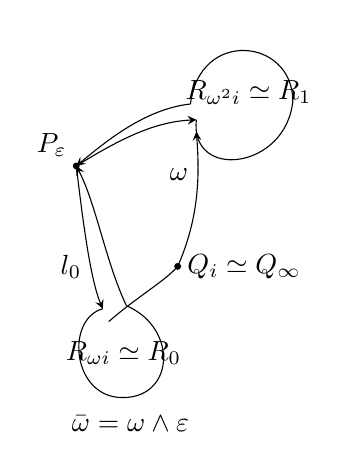
\begin{tikzpicture}[scale=1.25,>=stealth]
\coordinate (p) at (0,1.2);\coordinate (q) at (1.03,.18);
\fill (p) circle(1pt) node[above left]{$P_\varepsilon$};
\fill (q) circle(1pt) node[right]{$Q_i\simeq Q_\infty$};
\draw[->] (p) .. controls (.06,.7) and (.14,.05) .. (.27,-.25) node[pos=.65,left]{$l_0$};
\draw (.27,-.25) .. controls (-.1,-.35) and (-.05,-1.1) .. (.42,-1.15) .. controls (1,-1.2) and (1.05,-.45) .. (.51,-.22);
\draw[->] (.51,-.22) .. controls (.3,.22) and (.2,.82) .. (p);
\draw[->] (p) .. controls (.45,1.48) and (.8,1.65) .. (1.22,1.67);
\draw (1.22,1.67) .. controls (1.15,1.05) and (2.13,1.16) .. (2.2,1.86) .. controls (2.2,2.5) and (1.25,2.6) .. (1.16,1.83);
\draw[->] (1.16,1.83) .. controls (.7,1.78) and (.3,1.45) .. (p);
\draw (.33,-.38) .. controls (.63,-.12) and (.9,.03) .. (q);
\draw[->] (q) .. controls (1.26,.7) and (1.25,1.15) .. (1.22,1.55) node[pos=.65,left]{$\omega$};
\node at(.48,-.7){$R_{\omega i}\simeq R_0$};
\node at(1.75,1.95){$R_{\omega^2i}\simeq R_1$};
\node[below]at(.55,-1.24){$\bar\omega=\omega\wedge\varepsilon$};
\end{tikzpicture}}
On trouve de $=$, pour un autom qui renverse l'orientation de $\sigma$, i.e. pour un
\[
\widetilde\sigma_\infty:\quad\begin{array}{rcl}0&\longrightarrow&1\\1&\longrightarrow&0\\\infty&\longrightarrow&\infty\end{array}\qquad\deleted{\unsure{la}\ \illegible{1}}\bar\omega\longmapsto\bar\omega'
\]
\deleted{$\unsure{\widetilde\sigma_\infty}$}
\[
g_0=\widetilde\sigma_\infty\qquad r'=r\sigma_\infty=(\deleted{\unsure{\omega}}i,\omega',\bar\omega').
\]
d'où
\[
(41)\qquad\psi_\varepsilon^{\deleted{\unsure{\omega}}i,\omega'}=\inserted{\widetilde\sigma_i\circ\psi_\varepsilon^{i,\omega}=}\psi_\varepsilon^{i,\omega}\circ\widetilde\sigma_\infty
\]
($\widetilde\sigma_i$ est la symétrie p.r. du grand cercle méridien passant par $Q_i$)
\margin{57}

\scanpage{59}
\mspage{10}
Passons au cas de $Q_i$ -- la définition évidente \deleted{\unsure{géométrique}} des
\[
\psi_r=\psi_i^{\omega,\varepsilon}:\quad\Pi_{0,3}-\Pi_i\deleted{(\unsure{Q_i})}
\]
est
\[
\inserted{\psi_r=}\psi_i^{\omega,\varepsilon}=\Pi_1(\underbrace{u_{i,\omega,\varepsilon}}_{u_r};Q_\infty)
\]
\margin{\uline{NB} on identifie la \inserted{source $\Pi_1(U_{0,3};Q_\infty)$} \deleted{\unsure{source}} à $\Pi_{03}\stackrel{\mathrm{def}}=\Pi_1(U_{0,3};P_+)$ à l'aide du chemin standart $d_\infty^+$ de $P_+$ à $Q_\infty$.}
\unsure{Donc} $u_r=u_{i,\omega,\varepsilon}$ est l'unique isom de $U_{0,3}$, \inserted{dans $\Sigma^*$} qui transforme le repère \deleted{fixé} standart $(\infty,\omega_0=+1,\bar\omega_0=+1\text{ donc }\varepsilon=\omega_0\wedge\bar\omega_0=+1)$ en $r$ i.e. qui transforme $P_+$ en $P_\varepsilon$, $Q_0$ en $Q_i$, $Q_1$ en $Q_{\omega i}$. \deleted{On} Les épinglages \deleted{\unsure{par un repère fixé}} \inserted{$\psi_i^{\omega,\varepsilon}$ ($i$ fixé, $\omega,\varepsilon$ variables)} de $\Pi_i$ correspondent aux $u_r$ qui transforment $Q_0$ en $Q_i$, ils sont donc déterminés par composition avec des éléments
\[
g_0\in\Gamma_0=\mathcal G_3\times\{1,\tau\}
\]
qui stabilisent $Q_0$ -- ces éléments \deleted{engendrent} font un groupe $\simeq\mathbb Z/2\times\mathbb Z/2$ engendré par $\sigma_\infty,\tau$, \deleted{et} On trouve encore
\[
\psi_{r'}^{\deleted{\unsure{\omega}}}=\psi_r\circ\deleted{\unsure{\psi}}\Pi_1(g_0;Q_\infty)\quad\text{si }r'=r\circ g_0
\]
où ici $\psi_{r'},\psi_r$ désignent les iso. d'épinglage relatifs à $Q_i$. Il suffit d'expliciter ces formules dans les cas de $g_0=\sigma_\infty,g_0=\tau$, ce qui revient à calculer leur effet sur $\deleted{\unsure{\Pi_{0,3}=}}\Pi_1\deleted{\unsure{\varepsilon}}(U_{0,3};R_\infty)$, quand on identifie celui-ci à $\Pi_{03}=\Pi_1(U_{0,3};P_+)$, grâce au chemin $d_\infty^+$ de $P_+$ à $Q_\infty$. On sait que l'on peut
\margin{58}

\scanpage{60}
$\operatorname{int}(\sigma_\infty),\operatorname{int}\sigma\tau_\infty)$,
\inserted{Or dans ce cas $g_0=\tau_\infty$ resp. $g_0=\sigma_\infty$, \deleted{donc} \inserted{on} trouve $r'=(i,\omega,\varepsilon')$ resp. $r'=(i,\omega',\varepsilon')$, donc}
\[
(39)\qquad\begin{cases}
\psi_i^{\omega,\varepsilon'}=\tau\circ\psi_i^{\omega,\varepsilon}=\psi_i^{\omega,\varepsilon}\circ\tau_\infty\\[5pt]
\psi_i^{\omega',\varepsilon'}=\underbrace{\sigma_i}_{\substack{\text{transposition}\\\in\mathcal G_J\text{ qui}\\\text{fixe }i}}\circ\psi_i^{\omega,\varepsilon}=\psi_i^{\omega,\varepsilon}\circ\sigma_\infty
\end{cases}
\]
donc en composant
\[
(40)\qquad\psi_i^{\omega',\varepsilon\deleted{\unsure{'}}}=\deleted{\varepsilon}\underbrace{\widetilde\sigma_i}_{\substack{\tau\sigma_i\\\text{symétrie}\\\text{autour du}\\\text{grand cercle}\\\text{passant par}\\P_\varepsilon,P_{\varepsilon'},Q_i}}\circ\psi_i^{\omega,\varepsilon}=\psi_i^{\omega,\varepsilon}\circ\widetilde\sigma_\infty
\]
Dans tous ces calculs, suivant sans doute d'anciennes habitudes, j'ai privilégié les $P_\varepsilon$ et les $Q_i$ comme p\textsuperscript{ts} base -- alors que pour le travail que j'ai à faire, ce sont les points $R_i^\omega$ qui sont les plus cruciaux, \unsure{où|car} les calculs faits en ces p\textsuperscript{ts} capturent directement les phénomènes de ``monodromie'' autour des ``trous'' $R_i$. Je vais réparer cette négligence, en introduisant, en
\margin{59}

\scanpage{61}
\mspage{11}
plus des $\deleted{\widetilde{\unsure{\Pi|\Sigma}}_\omega}\Pi_\omega$ et $\deleted{\widetilde{\unsure{\Pi|\Sigma}}_i},\Pi_i$, des régions
\[
\widetilde\Sigma_r=\widetilde\Sigma_{\deleted{\unsure{r}}i\deleted{\unsure{\omega}}}^{\omega,\varepsilon}
\]
associés aux repères $r=(i,\omega,\deleted{\bar\omega}\varepsilon)$ de $(J,\uline{\varepsilon})$ (ou ce qui revient au $=$, de $(J,\uline{\bar\omega})$), qu'on peut identifier, géométriquement, aux \inserted{douze} triangles-drapeaux, \inserted{$D_r=P_\varepsilon Q_iR_{\omega i}$} correspondants à la subdivision barycentrique standart de la carte dans $\Sigma$ définie par l'équateur $\Sigma_{\mathbb R}$ et par les trois points $R_i$ sur celui-ci.
\figure{
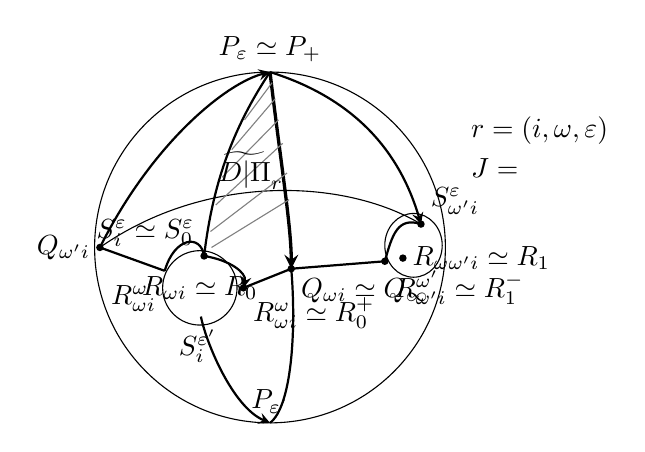
\begin{tikzpicture}[scale=1.35,>=stealth]
\coordinate (N) at(0,1.65);\coordinate (S)at(0,-1.65);\coordinate (L)at(-1.6,0);\coordinate (Q)at(.2,-.2);\coordinate (T)at(1.25,-.1);\coordinate (A)at(-.62,-.08);\coordinate (B)at(-.25,-.38);\coordinate (C)at(1.08,-.13);\coordinate (D)at(1.42,.22);
\draw[thin] (0,0)circle(1.65);
\draw[thin] (L) .. controls(-.6,.7)and(.7,.65)..(D);
\draw[->,thick] (L)..controls(-1.1,1.0)and(-.4,1.55)..(N);
\draw[->,thick] (N)..controls(.8,1.4)and(1.22,.9)..(D);
\draw[thick] (N)..controls(-.4,1.05)and(-.55,.5)..(A);
\draw[->,very thick] (N)..controls(.1,.8)and(.2,.2)..(Q);
\draw[thick] (Q)..controls(.25,-.8)and(.2,-1.5)..(S);
\draw[->,thick] (-.65,-.65)..controls(-.6,-.9)and(-.35,-1.5)..(S);
\draw[thick] (L)--(-.99,-.22);\draw[thick] (B)--(Q)--(C);
\draw[->,thick] (-.99,-.22)..controls(-.9,.1)and(-.65,.13)..(A)..controls(-.37,-.12)and(-.22,-.24)..(B);
\draw[thin] (-.66,-.38)circle(.35);
\draw[thick] (C)..controls(1.15,.12)and(1.2,.29)..(D);
\draw[thin] (1.35,.02)ellipse(.27 and .3);
\foreach \a/\b/\c/\d in {-.56/.15/.16/.7,-.51/.4/.12/.98,-.45/.66/.08/1.2,-.36/.92/.05/1.4,-.24/1.2/.02/1.55,-.55/.0/.18/.45}{\draw[thin,gray](\a,\b)--(\c,\d);}
\node at(-.18,.72){$\widetilde{\unsure{D|\Pi}}_r$};
\node[above] at(N){$P_\varepsilon\simeq P_+$};\node[above]at(S){$P_{\varepsilon'}$};
\node[left]at(L){$Q_{\omega'i}$};\node[below right]at(Q){$Q_{\deleted{\unsure{\omega}}i}\simeq Q_\infty$};
\node[above left]at(A){$S_i^\varepsilon\simeq S_0^\varepsilon$};\node[below]at(-.68,-.68){$S_i^{\varepsilon'}$};
\node[below left]at(-.98,-.2){$R_{\omega i}^{\omega'}$};
\node[below right]at(B){$R_{\omega i}^\omega\simeq R_0^+$};
\node at(-.66,-.38){$R_{\deleted{\unsure{\omega}}i}\simeq\deleted{\unsure{R_0}}$};
\node[below right]at(C){$R_{\omega'i}^{\omega'}\simeq R_1^-$};
\node[above right]at(D){$S_{\omega'i}^\varepsilon$};
\node[right]at(T){$R_{\deleted{\unsure{\omega}}\omega'i}\simeq R_1$};
\node[right]at(1.8,1.1){$r=(i,\omega,\varepsilon)$};\node[right]at(1.8,.75){$J=$};
\fill(L)circle(1pt);\fill(Q)circle(1pt);\fill(A)circle(1pt);\fill(B)circle(1pt);\fill(C)circle(1pt);\fill(D)circle(1pt);\fill(T)circle(1pt);
\end{tikzpicture}}
Le ``tronc'' \inserted{sur $\widetilde\Sigma$} au sens évident d'un tel triangle est un quadrilatère $\widetilde D_r$
\[
P_\varepsilon Q_{\omega'i}R_i^\omega S_i^\varepsilon\simeq P_+Q_\infty R_0^+S_0^+.
\]
On aura à travailler, au ``voisinage'' immédiat'' de ces \deleted{repères} \inserted{drapeaux} \deleted{\unsure{triangles des}} $\widetilde\Sigma_r$, avec les symétriques de $\Sigma_r$ p.r. à ses trois côtés, et se trouve sur $\widetilde\Sigma$, \deleted{\unsure{pour ce qui}} ce qui conduit à regarder la réunion de $\Sigma_r$ avec ses trois frères
\[
\tau(\Sigma_r),\widetilde\sigma_i(\Sigma_r),\widetilde\sigma_{\omega i}(\Sigma_r)
\]
(qui \inserted{resp.} correspondent, sur la sphère standart avec le repère correspondant au triangle $P_+Q_\infty R_0$, à $\tau,\widetilde\sigma_\infty,\widetilde\sigma_0$) et sur $\widetilde\Sigma$ à prendre
\[
(41)\qquad\widetilde\Sigma_r=\widetilde\Sigma_i^{\omega,\varepsilon}=\widetilde D_r\cup\tau(\widetilde D_r)\cup\widetilde\sigma_i(\widetilde D_r)\cup\widetilde\sigma_{\omega i}(\Sigma_+)
\]
limités par le contour
\[
P_\varepsilon Q_{\omega'i}R_{\omega i}^{\omega'}S_i^\varepsilon R_{\omega i}^{\omega}S_i^{\varepsilon'}P_{\varepsilon'}Q_iR_{\omega'i}^{\omega'}S_{\omega'i}^\varepsilon P_\varepsilon
\]
\margin{60}

\scanpage{62}
correspondant, sur la sphère standart, à la région ci-contre, délimitée par le contour
\[
P_+Q_1R_0^-S_0^+R_0^+S_0^-P_-Q_\infty R_1^-S_1^+P_+
\]
\figure{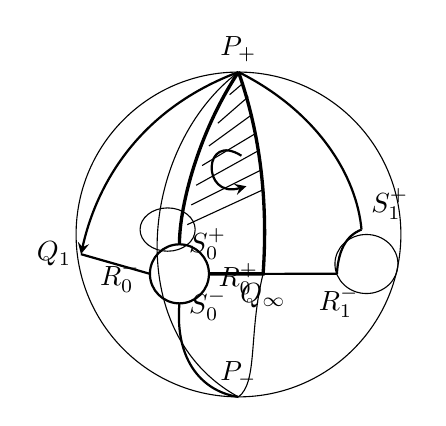
\begin{tikzpicture}[scale=1.25,>=stealth]
\coordinate(N)at(0,1.65);\coordinate(S)at(0,-1.65);\coordinate(L)at(-1.6,-.2);\coordinate(Q)at(.25,-.4);
\draw[thin](0,0)circle(1.65);
\draw[thin](N)..controls(-1,.9)and(-1.2,-1)..(S);
\draw[->,thick](N)..controls(-1.2,1.2)and(-1.5,.25)..(L);\draw[thick](L)--(-.9,-.4);
\draw[very thick](N)..controls(-.4,1.05)and(-.6,.3)..(-.6,-.1);
\draw[very thick](N)..controls(.23,1)and(.3,.3)..(Q)--(-.3,-.4);
\draw[thick](Q)--(1,-.4);\draw[thick](N)..controls(.8,1.25)and(1.2,.6)..(1.25,.05);
\draw[thick](-.6,-.4)circle(.3);\draw[thin](1.3,-.3)ellipse(.32 and .3);
\draw[thick](1,-.4)..controls(1.02,-.05)and(1.18,.02)..(1.25,.05);
\draw[thin](-.72,.05)ellipse(.28 and .22);
\draw[thick](-.6,-.7)..controls(-.65,-1.3)and(-.35,-1.6)..(S);
\draw[thin](Q)..controls(.1,-1)and(.2,-1.5)..(S);
\foreach \a/\b/\c/\d in {-.52/.1/.24/.45,-.48/.3/.22/.65,-.43/.5/.2/.85,-.37/.7/.18/1.03,-.3/.9/.14/1.22,-.21/1.13/.1/1.4,-.09/1.42/.05/1.54}{\draw[thin](\a,\b)--(\c,\d);}
\node[above]at(N){$P_+$};\node[above]at(S){$P_-$};\node[left]at(L){$Q_1$};\node[below]at(Q){$Q_\infty$};
\node[left]at(-.9,-.43){$R_0^-$};\node[right]at(-.3,-.45){$R_0^+$};\node[right]at(-.6,-.1){$S_0^+$};\node[right]at(-.6,-.72){$S_0^-$};
\node[below]at(1.02,-.43){$R_1^-$};\node[above right]at(1.25,.05){$S_1^+$};
\draw[->,thick] (.03,.8)..controls(-.36,1.05)and(-.38,.36)..(.08,.49);
\end{tikzpicture}}
Les régions $\widetilde\Sigma_r$ sont permutées de façon simplement transitive par $\Gamma=\mathcal G_J\times(1,\tau)$. Elles sont simplement connexes, et permettent donc de définir des
\[
\deleted{(42)}\qquad\Pi_r=\Pi_i^{\omega\varepsilon}=\Pi_1(\widetilde\Sigma;\widetilde\Sigma_r)=\Pi_1(\Sigma^*;\Sigma_r^*)
\]
\deleted{et des iso} \deleted{\unsure{qui|groupes}} mais qui sont reliés par un syst. transitif d'iso. à l'aide du gr. de $\Gamma$, de sorte qu'on peut identifier tous ces groupes entre eux. En fait, on trouve des isom. d'épinglage
\[
(42)\qquad\Psi_r:\Pi_{0,3}\longrightarrow\Pi_r=\unsure{\Pi_i|\Pi}^{\omega,i}=\Pi_1(\widetilde\Sigma;\widetilde\Sigma_r)
\]
($\psi_r$ majuscule

\deleted{en \unsure{identifiant|identi}}
en composant
\diagram{\begin{tikzcd}[ampersand replacement=\&,column sep=large]
\Pi_{03}\arrow[r,shorten >=1.7em]\arrow[r,"\psi_r=\psi_\varepsilon^{\omega,i}"]\&\begin{array}{c}\Pi_1(\widetilde\Sigma,P_\varepsilon)\\\simeq\Pi_1(\Sigma^*,P_\varepsilon)\end{array}\arrow[r,leftrightarrow,"\varphi_r^{-1}"]\&\Pi_r
\end{tikzcd}}
où \deleted{$\unsure{\varphi}$}
\[
\varphi_r:\Pi_r\longrightarrow\Pi_\varepsilon=\Pi_1(\widetilde\Sigma,P_\varepsilon)
\]
est ``\unsure{la'|l'}isomorphisme de transition'' correspondant à la région $1$-connexe $\Sigma_r$, et au point $P_\varepsilon$ de $\Sigma_r$.
\margin{61}

\scanpage{63}
\mspage{12}
La donnée d'un $R_i^\omega$, \inserted{qu'on va écrire $R_{\omega i}^{\omega}$, équivaut à} celle d'un repère \inserted{$r=(i,\omega)$} de $J$, et définit \uline{deux} \deleted{rég} régions $\widetilde D_r$ qui le contiennent, correspondant aux deux repères de $(J,\uline{\varepsilon})$ qui prolongent $r$ -- et il y a donc deux régions correspondantes $\widetilde\Sigma_r$, qui sont les seules qui contiennent $R_i^\omega$ comme \uline{point intérieur} (NB. dans la région $\widetilde\Sigma_{r_\varepsilon}$ \unsure{standart|standard}, les deux autres points $R$ à part $R_0^+$, qui est intérieur, sont $R_0^-$ et $R_1^-$, qui ne le sont pas). Mais si la sphère $\Sigma$ est orientée i.e. si on s'est donné un élément marqué \inserted{$\bar\omega_+$} de $\uline{\bar\omega}=\uline{\omega}\wedge\uline{\varepsilon}$, ou encore un isom $\unsure{\uline{\varepsilon}|\uline{\omega}}\simeq\deleted{\unsure{\uline{\omega}}}\inserted{\uline{\varepsilon}}$, alors le point $R_i^\omega$ détermine un $\varepsilon$ \inserted{$\in\uline{\varepsilon}$} privilégié, par la condition que $\varepsilon$ corresponde à $\omega$ par $\uline{\omega}\simeq\uline{\varepsilon}$ ou encore que $\omega\wedge\varepsilon=\bar\omega_+$, ce qui signifie aussi que l'orientation $P_+S_0^+R_0^+Q_\infty P_+$ de la région $\deleted{\widetilde\Sigma_r}\widetilde D_r$ est \deleted{celle de} $\bar\omega_+$. Donc on peut alors identifier canoniquement, via $\unsure{\Psi_r|\psi_r}$, $\Pi_1(\widetilde\Sigma,R_i^\omega)$ à $\Pi_{0,3}$, par un iso (qui dépend du choix de l'orientation $\bar\omega_+$ de $\Sigma$)
\[
(43),\qquad\psi_i^\omega:\Pi_{03}\xrightarrow{\sim}\Pi_1(\widetilde\Sigma,R_i^\omega)
\]
\margin{62}

\scanpage{64}
de sorte qu'on aura \deleted{compatibilité} \inserted{commutativité} de
\diagram{\begin{tikzcd}[ampersand replacement=\&,column sep=large,row sep=large]
\&\Pi_{03}\arrow[dl,"\Psi_i^\omega"',"\deleted{\Pi_{03}}"]\arrow[dl,shift left=1.5pt,shorten <=2.5em]\arrow[d,"\psi_{\deleted{\unsure{\varepsilon}}i}^{\omega\deleted{\unsure{\varepsilon}}}"]\arrow[dr,"\psi_\omega^i"]\&\\
(44)\quad\Pi_0(\widetilde\Sigma,R_{\omega i}^\omega)\&\begin{array}{c}\Pi_1(\widetilde\Sigma,Q_i)\\=\Pi_i\end{array}\arrow[l,"b_i^{\omega'}(\cdot)"',"{\deleted{\unsure{\rightarrow}}}"{description,pos=.08}]\&\begin{array}{c}\Pi_1(\widetilde\Sigma,P_\omega)\\=\Pi_\omega\end{array}\arrow[l,"\varphi_{i\omega}=c_i^\omega(\cdot)"',"{\deleted{\unsure{\rightarrow}}}"{description,pos=.08}]
\end{tikzcd}}
où on a écrit $P_\omega$ au lieu de $P_\varepsilon$ (en identifiant $\uline{\omega}$ et $\uline{\varepsilon}$ grâce à $\bar\omega_+$) et $\psi_i^\omega$ au lieu de $\psi_i^{\omega,\omega}$, $\psi_\omega^i$ au lieu de $\psi_\omega^{i,\omega}$.

Le passage à expliciter est celui de
\diagram{\begin{tikzcd}[ampersand replacement=\&,column sep=large]
\deleted{R_{\omega i}}\Pi_i^\omega\simeq\Pi_1(\widetilde\Sigma,R_{\omega i}^{\omega})\&\text{à}\&\Pi_i^{\omega'}=\Pi_1(\widetilde\Sigma,R_{\omega'i}^{\omega'})\\
\Pi_{0,3}\arrow[u,"\psi_i^\omega","\sim"']\&\&\Pi_{03}\arrow[u,"\psi_i^{\omega'}","\sim"']
\end{tikzcd}}
\inserted{Via $\widetilde b_{i\omega}$.}
\figure{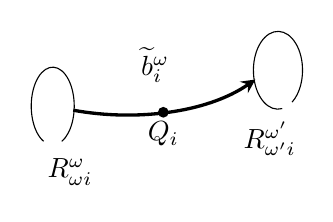
\begin{tikzpicture}[scale=1.3,>=stealth]
\draw(-.089,-.344)arc[start angle=245,end angle=-65,x radius=.21,y radius=.38];\draw(2.242,-.024)arc[start angle=280,end angle=-55,x radius=.24,y radius=.38];
\draw[->,very thick](.2,-.04)..controls(.8,-.15)and(1.5,-.07)..(1.98,.26);
\fill(1.08,-.06)circle(1.5pt)node[below]{$Q_i$};\node at(1,.4){$\widetilde b_i^\omega$};
\node[below]at(.17,-.42){$R_{\omega i}^{\omega}$};\node[below]at(2.12,-.06){$R_{\omega'i}^{\omega'}$};
\end{tikzpicture}}
On trouve par la commutativité (44) et par la dernière formule (39) qu'on a
\deleted{$\widetilde b_{\omega i}$}
\[
(45)\qquad\widetilde b_i^\omega\bigl(\psi_i^\omega(\deleted{\unsure{g}}x)\bigr)=\psi_i^{\omega'}(\sigma_\infty(x).
\]
\margin{63}

\scanpage{66}
\margin{(\unsure{38|39} pages)}
\mspage{5}
Généralités sur les actions de groupes de Galois sur les compactifiés profinis de groupoïdes fondamentaux de variétés Alg. complexes
\margin{65}

\scanpage{67}
\mspage{1}
Soit $K$ un sous-corps du corps des complexes $\mathbb C$ -- des cas intéressants seront celui où $K=\mathbb Q$, ou $K$ extension finie de $\mathbb Q$, ou $K=\widetilde{\mathbb Q}$ extension abélienne maximale de $\mathbb Q$ dans $\mathbb C$ -- je serai intéressé en tous cas avant tout aux cas où $K$ est de t.f. sur $\mathbb Q$. (Le cas de $\widetilde{\mathbb Q}$ est un cas ``limite'' de tels cas, pour ne pas être gêné par les racines de $1\ldots$).

On s'intéresse aux schémas \inserted{$X$} de t.f. sur $K$, et aux espaces \inserted{analytiques} $X(\mathbb C)$ correspondants. Comme on s'intéresse aux invariants ``topologiques'' de $X,X(\mathbb C)$, on traitera les morphismes $X'-X$ qui induisent des homéomorphismes universels comme des iso -- en particulier les éléments nilpotents ne comptent pas -- une imm. fermée surjective sera traitée comme un iso.

Un langage commode est de considérer $X$ comme donné par l'espace analytique (ou $\overline{\mathrm m}$ seulement topologique) $X(\mathbb C)$, plus une \uline{structure} supplémentaire dessus : la structure de ``var. alg. sur $K$'', à coups de top. de Zariski, de faisceau des fonctions $K$-polynomiales etc. On écrira par la suite $X$ au lieu de $X(\mathbb C)$.

On distingue sur $X$ le groupoïde fondamental $\Pi_1(X)$ au sens topologique, et son compactifié profini $\widehat\Pi_1(X)$, qui \deleted{est \unsure{en un} sens} \inserted{peut} aussi être défini directement en termes du $\mathbb C$-schéma $X$. On a un foncteur ``d'inclusion''
\margin{66}

\scanpage{68}
\[
(1)\qquad\Pi_1(X)\longrightarrow\widehat\Pi_1(X)
\]
qui induit une bijection sur l'ens des objets \inserted{ou ``sommets''} -- s'identifiant à $X=X(\mathbb C)$ -- et qui \deleted{déf} pour tt $x\in X=X(\mathbb C)$, donne l'hom de groupes
\[
(2)\qquad
\begin{array}{ccc}
\operatorname{Aut}_{\Pi_1(X)}(x)&\longrightarrow&\operatorname{Aut}_{\widehat\Pi_1(X)}(x)\\
\Vert\ \text{déf}&&\Vert\ \text{déf}\\
\pi_1(X,x)&&\widehat\pi_1(X_{\mathrm{sch}},x)
\end{array}
\]
permettant d'identifier le $\pi_1$ algébrique au compactifié profini du $\pi_1$ ``topologique'' ou ``transcendant'' : \unsure{b}
\[
(3)\qquad\pi_1(X_{\mathrm{sch}},x)\simeq\widehat\pi_1(X,x).
\]
De $=$, pour $x,y\in X$, l'application
\[
\operatorname{Hom}_{\Pi_1(X)}(x,y)\longrightarrow\operatorname{Hom}_{\widehat\Pi_1(X)\deleted{\unsure{y}}}(x,y)
\]
\margin{On identifiera un élément de $\operatorname{Hom}_{\Pi_1}(x,y)$ avec son image dans $\operatorname{Hom}_{\widehat\Pi_1}(x,y)$, sans se préoccuper si l'application est injective ou non.}
permet d'identifier le deuxième ens, en tant que bi-torseur sur $(\widehat\pi_1(X,y),\widehat\pi_1(X,x))$ au bitorseur déduit \deleted{Hom} du premier ens par extension des groupes d'opérateurs par
\[
\pi_1(X,y)\longrightarrow\widehat\pi_1(X,y),\qquad\pi_1(X,x)\longrightarrow\widehat\pi_1(X,x).
\]
(ce couple d'homomorphismes satisfaisant \inserted{bien} à la condition requise pour que cette extension ait un sens\ldots).
\margin{à savoir (en termes de $(G,H),(G',H')$ et $G\to G',H\to H'$ : il existe un isom ext. $G'\xrightarrow{\sim}H'$ rendant commutatif le diagramme \deleted{\unsure{des bitorseurs}}
\diagram{\begin{tikzcd}[ampersand replacement=\&,column sep=large,row sep=large]
G\arrow[r,"\sim", "\substack{\text{défini par le}\\\text{bitorseur }(G,H)}"']\arrow[d]\&H\arrow[d]\\
G'\arrow[r,"\sim"]\&H'
\end{tikzcd}})}
Soit
\[
(5)\qquad\mathbf{\Gamma}_{\deleted{K}}=\mathbf{\Gamma}_K=\operatorname{Aut}_{K\text{-cor}}(\mathbb C),
\]
\margin{67}

\scanpage{69}
\mspage{2}
alors $\mathbf{\Gamma}$ opère non seulement sur \deleted{$X$} l'ens. $X$, mais aussi sur le groupoïde $\widehat\Pi_1(X)$, à cause du fait que celui-ci admet une définition purement schématique, ne faisant p intervenir la topologie de $\mathbb C$. Bien entendu, si $\lambda:\deleted{x} x\to y$ dans $\Pi_1$, alors pour $u\in\Gamma$, $u(\lambda)$ n'est p en général une flèche de $\Pi_1$ (de $u(x)$ vers $u(y)$) mais seulement de $\widehat\Pi_1$.

\deleted{Notation} Notation ${}^ux$ ($x\in X,u\in\mathbf{\Gamma}$) et \deleted{\unsure{``}}
\[
{}^u\lambda:{}^ux-{}^uy\qquad\text{si }\lambda:x\to y\quad(\text{dans }\widehat\Pi_1(X)).
\]
On a
\[
(6)\qquad\begin{cases}
{}^u(\operatorname{id}_x)=\operatorname{id}_{{}^ux}\qquad(x\in X)\\
{}^u(\mu\lambda)={}^u\mu\,{}^u\lambda
\end{cases}
\]
\diagram{\(\left(\begin{tikzcd}[ampersand replacement=\&,column sep=large]
x\arrow[r,"\lambda"]\&y\arrow[r,"\mu"]\&z\\
{}^ux\arrow[r,"{}^u\lambda"]\&{}^uy\arrow[r,"{}^u\mu"]\&{}^uz
\end{tikzcd}\right)\)}
Notre objet est d'essayer de ``déterminer'' autant que faire se peut cette action de $\mathbf{\Gamma}$. À vrai dire, si $\bar K$ est la clôture algébrique de $K$ dans $\mathbb C$, on s'intéressera surtout aux sous-groupoïdes de $\Pi_1(X)$ et $\widehat\Pi_1(X)$ induits sur l'ens d'objets $X_{\bar K}$, qu'on désignera par $\Pi_1(X_{\bar K}),\widehat\Pi_1(X_{\bar K})$ -- le deuxième est stable par l'action de $\mathbf{\Gamma}$, et si on pose
\[
(7)\qquad\Gamma=\operatorname{Aut}_{K\text{-cor}}(\bar K)=\operatorname{Gal}_{\bar K/K},
\]
de sorte que $\Gamma$ est un quotient de $\mathbf{\Gamma}$, l'action de $\mathbf{\Gamma}$ sur $\Pi_1(X_{\bar K})$ se fait à travers $\Gamma$. $\uparrow$
\margin{68}

\scanpage{70}
Pour décrire l'action d'un $u\in\mathbf{\Gamma}$ (resp $u\in\Gamma$) sur $\widehat\Pi_1(X)$ (resp. $\deleted{\unsure{\Pi}}\widehat\Pi_1(X_{\bar K})$), on prendra comme ``générateurs'' du groupoïde $\widehat\Pi_1$ des chemins provenant de $\Pi_1$. On aura, pour ${l}:x\to y$ dans $\Pi_1$, ${}^u{l}:{}^ux\to{}^uy$.

Si \deleted{\unsure{on suppose}} par la suite, pour simplifier, on se borne à des points $x,y\ldots$ rationnels sur $X$ -- i.e. qu'on travaille dans le sous-groupoïde $\widehat\Pi_1(X_K)$ formé des objets qui sont invariants sous $\mathbf{\Gamma}$ -- alors on aura
\[
(*)\qquad{}^u{l}:{}^ux=x\longrightarrow{}^uy=y,
\]
et on peut écrire, \deleted{f}..
\[
(8)\qquad\begin{cases}
{}^u{l}=g_{l}(u)\circ{l}={l}\circ f_{l}(u)\\
g_{l}(u)\in\widehat\pi_1(X,y)\\
f_{l}(u)\in\widehat\pi_1(X,x)
\end{cases}
\]
\deleted{$g_{l}(u)={}^u{l}\circ{l}^{-1}$}
\figure{\begin{tikzpicture}[x=2mm,y=2mm]
\node at(0,0){,};
\fill(.5,.8)circle(.07);\fill(.75,.55)circle(.07);\fill(1.25,.4)circle(.08);\fill(1.75,.08)circle(.045);
\fill[gray](1.16,-.08)circle(.04);\fill[gray](1.38,-.1)circle(.035);
\end{tikzpicture}}
\margin{On écrira aussi parfois $g_u({l})$ au lieu de $g_{l}(u)$, $f_u({l})$ pour $f_{l}(u)$.}
où $f_{l}(u),g_{l}(u),{}^u{l}$ se déterminent mutuellement, \deleted{$f_l(u)$ et $g_l(u)$} par les formules (8) et
\[
(9)\qquad\begin{cases}
f_{l}(u)={l}^{-1}\cdot{}^u{l},\quad g_{l}(u)={}^u{l}\cdot{l}^{-1}\\
g_{l}(u)={l}(f_{l}(u)),\quad f_{l}(u)={l}^{-1}(g_{l}(u))
\end{cases}
\]
On décrira l'action d'un $u\in\Gamma$ \inserted{sur un sous-groupoïde plein de $\Pi_1(X)$} à l'aide des éléments $f_{l}(u)$, ou $g_{l}(u)$, pour un syst. de générateurs convenable des \inserted{groupoïdes pleins} correspondants de $\Pi_1(X)$. Dans le cas d'un
\margin{69}

\scanpage{71}
\mspage{3}
sous-groupoïde induit sur une partie \uline{finie} \deleted{\illegible{1}} $I$ de $X_K$, on pourra trouver un nb fini de tels générateurs --- il suffit p.ex. de choisir un \deleted{\unsure{$x$}} $x_0\in I$, et choisir pour tt $x\in I\setminus x_0$ un chemin $l_x$ de $x_0$ à $x$, et de plus un syst. \inserted{fini} de générateurs $l_i$ de $\Pi_1(X,x_0)$.

\unsure{Il|Je} apparaît que sous des conditions assez générales (p.ex. si $X$ est une courbe alg. anabélienne) la connaissance de l'opération $u$ sur $\widehat{\Pi}_1(X_K,I)$ (\inserted{pour un} $u\in\Gamma$) \uline{suffit à} déterminer $u$ --- et la question se pose alors de voir comment la connaissance des invariants \inserted{disons} $g_{l_\alpha}(u)$ (pour un syst. générateur de flèches $l_\alpha$ de $\Pi_1(X,I)$) permet de retrouver les invariants $g_l(u)$ pour d'autres \inserted{$K$-}schémas $Y\ldots$.
\margin{\figure{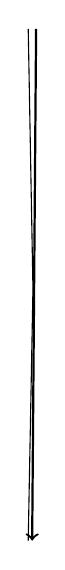
\begin{tikzpicture}[x=1mm,y=1mm]\draw (0,0)--(.6,32)--(0,65);\draw[->,line width=.8pt] (1,65)--(.5,0);\end{tikzpicture}}}

Quand il s'agit du $=$ schéma $X$, et qu'on s'intéresse à d'autres chemins $l:x\longrightarrow y$ $(x,y\in I)$ que les générateurs choisis $l_\alpha$, la formule donne en principe un moyen de reconstituer les $g_l(u)$ pour tout $l$, puisqu'il permet de retrouver les ${}^u l$, et que ${}^u l$ est multiplicatif en $l$. En termes des $g_l(u)$, \deleted{$=f_l(u)$}, la formule de multiplicativité (6) s'écrit, pour une situation
\margin{\uline{NB} pour le moment, on ne regarde que les $x\in X_K$ qui sont dans $I$, le syst fini de sommets choisi.}
\diagram{\begin{tikzcd}[ampersand replacement=\&,column sep=large]
x\arrow[r,"l'"] \& y\arrow[r,"{l\deleted{\unsure{''|'}}}"] \& z
\end{tikzcd}}
\[
(10)\qquad \unsure{g_{ll'}(ll'\deleted{u})|g_{ll'}(\deleted{ll'}u)}=g_l(u)\cdot l\bigl(g_{l'}(u)\bigr)
\qquad\text{soit }g_u(ll')=g_u(l)\cdot l\bigl(g_u(l')\bigr)
\]
\margin{70}

\scanpage{72}
et en termes des $f\ldots$ la formule, est. identique mais d'allure un peu moins sympathique
\[
(11)\qquad f_{ll'}(u)=l'^{-1}\bigl(f_l(u)\bigr)\cdot f_{l'}(u)
\qquad\text{i.e. }f_u(ll')=l'^{-1}f_u(l)\cdot f_u(l')
\]

\deleted{La formule (10) peut s'exprimer en disant que pour $l$ fixé, $u\in\Gamma$ variable,
\[
\unsure{(17)|(12)}\qquad g_l:\Gamma\longrightarrow\widehat{\pi}_1(X,y)
\]
est un $1$-cocycle sur $\Gamma$, à valeurs dans $\widehat{\pi}_1(X,y)$, relativement à l'action naturelle de $\Gamma$ sur $\widehat{\pi}_1(X,y)$. Bien entendu, le $\widehat{\pi}_1(X,y)$-torseur à gauche, \inserted{avec op. de $\Gamma$,} correspondant à ce $1$-cocycle, n'est autre que $\operatorname{Hom}_{\widehat{\Pi}_1(X)}(x,y)$, sur lequel $\widehat{\pi}_1(X,y)=\operatorname{Hom}_{\widehat{\Pi}_1(X)}(y,y)$ opère par composition.}

Pour un composé d'une \deleted{nb fini} suite finie composable de chemins
\diagram{\begin{tikzcd}[ampersand replacement=\&]
x_0\arrow[r,"l_1"]\&x_1\arrow[r,"l_2"]\&\cdots\&x_{n-1}\arrow[r,"l_n"]\&x_n
\end{tikzcd}}
la formule (10) prend la forme
\[
\unsure{(12)|(13)}\qquad
 g_{l_nl_{n-1}\cdots l_1}(u)=g_{l_n}(u)\cdot l_n\bigl(g_{l_{n-1}}(u)\bigr)\cdot l_nl_{n-1}\bigl(g_{l_{n-2}}(u)\bigr)\ldots
 \inserted{\cdot(l_n\cdots l_2)g_{l_1}(u))}
\]
Formule la plus \deleted{évidente} \inserted{simple} possible en somme de celles qu'on pourrait imaginer qui ait un sens. On va développer \deleted{encore} \inserted{un} contexte qui permette \deleted{mieux} d'écrire cette formule, ainsi que \deleted{(11)} la formule analogue en $f$ et les formules
\margin{71}

\scanpage{73}
\mspage{4}
(9) de passage de $f$ à $g$, sous une forme considérablement plus simple.

Soit $T$ un espace topologique \deleted{simplement} $1$-connexe, et
\[
(13)\qquad p:T\longrightarrow X
\]
une application continue \inserted{(le cas injectif sera le plus intéressant)}. Soit $T_K=p^{-1}(X_K)$.

Considérons \deleted{\unsure{$\Pi_1(T_K),\ \Pi_1$}}
\deleted{\unsure{Soient} $x,y\in T_K$}
\[
(14)\qquad\deleted{\unsure{\Pi_1(X)}}\ \Pi_1(X;T)=\pi
\]
alors pour tout $x\in T$ on a un isom canonique
\[
(15)\qquad\varphi_x:\pi\xrightarrow{\sim}\Pi_1(X,p(x))
\]
\inserted{de sorte que les $\Pi_1(X,p(x))$ sont munis d'un syst. transitif d'iso}
\margin{On désigne aussi par $\varphi_x$ (15) le prolongement aux complétés profinis\ldots}
et pour $x,y\in T$, l'unique \deleted{élément} \inserted{flèche} de \unsure{\deleted{Hom}|Hom} $x:y$ de $\Pi_1(T)$ donne \inserted{par $p$} une flèche canonique
\[
(16)\qquad l_{y,x}:p(x)\longrightarrow p(y)\qquad\text{dans }\Pi_1(X)
\]
(NB cette flèche dépend du choix de $x,y$ au dessus de $px,py$ --- mais naturellement $p$ sera injective).

Moyennant les iso (15), on peut considérer $f_{l_{y,x}}(u)$ et $g_{l_{y,x}}(u)$ (\inserted{du moins} si $x,y\in T_K$ i.e. $p(x),p(y)\in X_K$) comme des éléments du $=$ groupe $\pi$ (14), \deleted{soit} et en fait ces deux éléments se réduisent à un seul et $=$ élément, soit
\[
\begin{array}{c}
\unsure{(17)}\qquad g_{y,x}^{T/X}(u)=g_{y,x}^{p}(u)=\varphi_y^{-1}\bigl(g_{l_{y,x}}(u)\bigr)=\varphi_x^{-1}\bigl(f_{l_{y,x}}(u)\bigr)\\
\begin{tikzpicture}[baseline=-.4ex]\node[rotate=90]{$\in$};\end{tikzpicture}\\
\pi=\Pi_1(X;T)
\end{array}.
\]
\margin{72}

\scanpage{74}
Les formules (10) (11) se réduisent donc à la formule
\[
(18)\qquad g_{zy}(u)g_{yx}(u)=g_{zx}(u)\qquad x,y,z\in T_K
\]
\margin{On a laissé tomber l'exposant $T$ : $g_{y,x}^{T/X}$, qui est nécessaire surtout si $T\subset X\ldots$}
et la formule (12) à la formule itérée de celle-ci
\[
(19)\qquad g_{x_n,x_0}=g_{x_n,x_{n-1}}\,g_{x_{n-1},x_{n-2}}\cdots g_{x_1,x_0}
\]
--- quant aux formules de passage (9), elles \deleted{\unsure{tombent}} disparaissent !

Bien entendu, les invariants $g_l(u)$ \inserted{ou $f_l(u)$} peuvent être considérés comme décrits par des invariants précédents du type $g_{y,x}^T$, en prenant \deleted{\unsure{$T$}} p.ex. $T=[0,1]$, $p$ une application $[0,1]\longrightarrow X$ \unsure{donnant} naissance \deleted{au} chemin $l$ (plutôt, à la classe de chemins\ldots) de sorte qu'on aura
\[
(20)\qquad f_l(u)=\varphi_x\bigl(g_{y_0,x_0}^T(u)\bigr),\qquad g_l(u)=\varphi_y\bigl(g_{y_0,x_0}^T(u)\bigr)
\]
\deleted{$x_0=0\in T,\ y_0$}
\[
x_0=0,\ \deleted{\unsure{0}}\ y_0=1\qquad\in T=[0,1].
\]
\margin{Autre exemple ``illuminant'' : si $x_0\in X_K$ fixé, pour les $y\in X_K$ ``voisins'' de $X$, choisissons des chemins ``directs'' $x_0\longrightarrow y$ (``voisins'' de $x_0$) on trouve des invariants $g_{y,x_0}(u)\in\Pi_1(X,x_0)$.}

\deleted{La relation de $1$-cocycle}
\deleted{Bien entendu,}
\deleted{On peut}
Pour comparer les invariants $g_{x,y}^T$ associés à différents espaces $1$-connexes au dessus de $X$, il suffit de regarder le cas où on a un diag. comm.
\diagram{\begin{tikzcd}[ampersand replacement=\&,column sep=large]
T\arrow[rr,"f"]\arrow[dr,"p"'] \&\& T'\arrow[dl,"p'"]\\
\&X\&
\end{tikzcd}}
\[
(21)
\]
d'où $f_K:T_K\longrightarrow T'_K$,
\margin{73}

\scanpage{75}
\mspage{5}
et un homomorphisme
\[
(22)\qquad\pi=\Pi_1(X;T/X)\overset{\psi=\Pi_1(f)}{\longrightarrow}\pi'=\Pi_1(X,T'/X)
\]
Ceci dit, si $x,y\in T_K$, d'où $x'=f(x),y'=f(y)\in T'_K$, on aura
\[
(23)\qquad g_{y',x'}^{T'}(u)=\psi\bigl(g_{y,x}^T(u)\bigr)
\qquad(x'=f(x),y'=f(y),\psi=\Pi_1(f))
\]

Conséquence pratique : Supposons $X=\bigcup_{\alpha\in A}T_\alpha$, les $T_\alpha$ $1$-connexes, d'où des \deleted{fonctions} \inserted{groupes}
\[
\deleted{\unsure{g_\alpha^{T_i}|f_\alpha^{T_i}}:\unsure{\Gamma\times}T_{iK}\times T_{iK}\longrightarrow}
\]
\[
(24)\qquad \pi_\alpha\overset{\text{déf}}{=}\Pi_1(X,T_\alpha)
\]
et des fonctions
\[
(25)\qquad\left\{\begin{aligned}
T_{\alpha K}\times T_{\alpha K}\times\Gamma&\longrightarrow\pi_i\\
(x,y,u)&\longmapsto g_{y,x}^{T_\alpha}(u)\overset{\text{déf}}{=}g_{y,x}^{\alpha}(u)
\end{aligned}\right.
\]
satisfaisant la formule de multiplicativité (19).

Pour relier les fonctions entre elles, \deleted{il faut} on \deleted{considère \unsure{les groupes} pour} \inserted{note que pour} $T_\alpha\subset T_\beta$, on a
\[
(26)\qquad\deleted{\unsure{\forall}}\ \varphi_{\beta\alpha}:\pi_\beta\longrightarrow\pi_\alpha
\]
et les relations
\[
(27)\qquad\deleted{g}\quad g_{y,x}^{\beta}(u)=\varphi_{\beta\alpha}\bigl(g_{y,x}^{\alpha}(u)\bigr)\qquad\begin{gathered}x,y\in T_{\alpha K}\\u\in\Gamma\end{gathered}
\]
Supposons que l'ens d'indices $\mathbb{I}$, avec sa relation d'ordre induite par l'inclusion $T_\alpha\subset T_\beta$, soit tel que \deleted{$\Pi_0(I)\unsure{\leftrightarrow|\longrightarrow}\Pi_0(X)$ est bijectif}
\[
(28)\qquad\forall\alpha,\beta\in I,\quad\text{on a}\quad T_\alpha\cap T_\beta=\bigcup_{\gamma\le\alpha,\beta}T_\gamma
\]
\[
\deleted{\Pi_0(I)\xrightarrow{\sim}\Pi_0(X)}
\]
\margin{74}

\scanpage{76}
\deleted{(enfin la surjectivité est acquise) que $T_\alpha,T_\beta$ sont dans une $=$ comp. connexe de $X$, il existe une ``chaîne'' d'\uline{indices}
\[
i_0=i,\ i_1,\ldots,i_n=j
\]
telle que pour deux indices consécutifs $k=i_{\unsure{r|\nu}}$, $k'=i_{\unsure{r|\nu}+1}$, on ait $T_k\subset T_{k'}$ ou $T_{k'}\subset T_k$.}
\margin{Supposons de plus que les intérieurs des $T_\alpha$ recouvrent $X$ \uline{ou} que les $T_\alpha$ soient fermés (\deleted{et} $A$ fini) Alors $\Pi_0(A)\xrightarrow{\sim}\Pi_0(X)$. Mieux ---}

Supposons de plus \inserted{que les intérieurs des $T_i$ recouvrent $X$,} \deleted{que les $T_i$ s'} \inserted{\uline{Ceci posé,}} je dis que la connaissance des (pour $u$ fixé) des $g_{y,x}^\alpha(u)\in\pi_\alpha$ \inserted{($\alpha\in A,y,x\in T_\alpha$)} permet de retrouver tous les invariants $g_l(u)$ (ou $f_l(u)$). En effet, il suffit de voir que les flèches $l_{y,x}^\alpha=p_\alpha(l_{y,x})$ ($\alpha\in I$, $x,y\in T_\alpha$, $p_\alpha:T_\alpha\hookrightarrow X$ l'inclusion) \deleted{eng} forment un syst. de générateurs du groupoïde $\Pi_1(X_K)$\deleted{\unsure{$x_0$}} --- \inserted{tous} \unsure{les|des} \deleted{obj} sommets sont obtenus en tous cas, et on trouve une application bijective sur les $\Pi_0$ (du groupoïde engendré par les gén. $l_{y,x}^\alpha$ \inserted{($\alpha\in I,x,y\in T_{\alpha K}$) et les relations $l_{y,x}^{\beta}=\varphi_{\beta\alpha}(l_{y,x}^{\alpha})$} et de $\Pi_1(X_K)$), il faut voir qu'on a une application surjective sur les $\Pi_1$.

Quand les intérieurs des $T_{\inserted{\alpha}\deleted{\unsure{\alpha|i}}}$ recouvrent $X$, il suffit de noter que la connaissance des $g_{y,x}^{\alpha}(u)$ nous donne les $g_{y,x}(u)$ (sans exposant $\alpha$ !) pour $x,y$ points ``voisins'' sur $X$,
\margin{75}

